\chapter{Methodology}

You are expected to be methodical in your work, so that it could and can be
reproduced and replicated by others to verify your results.
If you are clear in your methodology, you will have a better chance of someone
building on your work \cite{villaneuva18}.
That will lead to more people being interested in what you have done, and will
give you a higher profile.
Remember that undergraduate students will sometimes do projects based on
academic research, so it's a good idea to be explicit enough that they can
easily replicate your results.

It is important that you demonstrate that you were methodical from the start.
While it is tempting to play around with various algorithms or techniques
before you really sit down to work.
If you take five minutes beforehand to think through what you are about to do
and write it down, you will quickly build up a portfolio of writing and results
that can go into your thesis.
There is often very little pracitcal difference between being methodical and
playing around -- it's largely in your attitude while you are doing the work.

Note that \LaTeX has a lot of nice functionality for creating various types of
plots and diagrams.
Check out the nice graphs in Figure \ref{tikz:graphs}.

\lipsum[26]

\begin{figure}[ht]
  \centering
  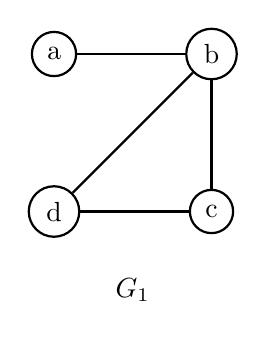
\begin{tikzpicture}
    \begin{scope}[every node/.style={circle,thick,draw}]
      \node (a) at (0,2) {a};
      \node (b) at (2,2) {b};
      \node (c) at (2,0) {c};
      \node (d) at (0,0) {d};
    \end{scope}
    \begin{scope}[every edge/.style={draw=black,thick}]
      \path (a) edge (b);
      \path (b) edge (c);
      \path (b) edge (d);
      \path (c) edge (d);
    \end{scope}
    \node () at (1,-1) {$G_1$};
  \end{tikzpicture}
  \hspace{1.5cm}
  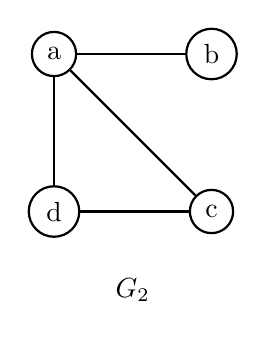
\begin{tikzpicture}
    \begin{scope}[every node/.style={circle,thick,draw}]
      \node (1) at (0,2) {a};
      \node (2) at (2,2) {b};
      \node (3) at (2,0) {c};
      \node (4) at (0,0) {d};
    \end{scope}
    \begin{scope}[every edge/.style={draw=black,thick}]
      \path (1) edge (2);
      \path (1) edge (3);
      \path (1) edge (4);
      \path (3) edge (4);
    \end{scope}
    \node () at (1,-1) {$G_2$};
  \end{tikzpicture}
  \caption{Nice pictures}
  \label{tikz:graphs}
\end{figure}

\subsection{Vector Spaces}

A \textbf{vector space} $V$ over a field $\mathbb{F}$ is a set equipped with two operations:

\begin{itemize}
    \item Vector addition: $+: V \times V \rightarrow V$, denoted as $(\mathbf{v}, \mathbf{w}) \mapsto \mathbf{v} + \mathbf{w}$.
    \item Scalar multiplication: $\cdot: \mathbb{F} \times V \rightarrow V$, denoted as $(\lambda, \mathbf{v}) \mapsto \lambda \mathbf{v}$.
\end{itemize}

These operations satisfy the following properties for all $\mathbf{u}, \mathbf{v}, \mathbf{w} \in V$ and $\lambda, \mu \in \mathbb{F}$:

\begin{enumerate}
    \item \textbf{Addition is commutative}: $\mathbf{u} + \mathbf{v} = \mathbf{v} + \mathbf{u}$.
    \item \textbf{Addition is associative}: $(\mathbf{u} + \mathbf{v}) + \mathbf{w} = \mathbf{u} + (\mathbf{v} + \mathbf{w})$.
    \item \textbf{Additive identity}: There exists a vector $\mathbf{0} \in V$ such that $\mathbf{v} + \mathbf{0} = \mathbf{v}$ for all $\mathbf{v} \in V$.
    \item \textbf{Additive inverse}: For every vector $\mathbf{v} \in V$, there exists a vector $-\mathbf{v} \in V$ such that $\mathbf{v} + (-\mathbf{v}) = \mathbf{0}$.
    \item \textbf{Scalar multiplication is distributive over vector addition}: $\lambda (\mathbf{v} + \mathbf{w}) = \lambda \mathbf{v} + \lambda \mathbf{w}$.
    \item \textbf{Scalar multiplication is distributive over scalar addition}: $(\lambda + \mu) \mathbf{v} = \lambda \mathbf{v} + \mu \mathbf{v}$.
    \item \textbf{Scalar multiplication is associative}: $(\lambda \mu) \mathbf{v} = \lambda (\mu \mathbf{v})$.
    \item \textbf{Scalar multiplication identity}: $1 \cdot \mathbf{v} = \mathbf{v}$, where $1$ is the multiplicative identity in $\mathbb{F}$.
\end{enumerate}